\chapter{System DIMAC-EK}

Niniejsza praca magisterska związana jest bezpośrednio z systemem sterowania urządzeniami energetyki kolejowej o nazwie DIMAC-EK. Niniejszy rozdział zawiera pobieżny opis systemu, by przybliżyć czytelnikowi tematykę pracy.

\section{Funkcje}

System DIMAC-EK jest złożonym rozwiązaniem zajmującym się sterowaniem automatyką kolejową\cite{dimacek-katalog}. Jego głównym zadaniem jest zapewnienie drożności tras kolejowych podczas trudnych warunków pogodowych oraz dostarczanie pomiarów związanych z tą funkcją. Czynności te dotyczą głównie okresu zimowego, gdy mróz oraz śnieg jest w stanie blokować działanie rozjazdów kolejowych oraz tarasować przejazd. W skład systemu wchodzą następujące elementy:

\begin{itemize}
\item oświetlanie oraz osuszanie terenów kolejowych,
\item ochrona antywłamaniowa i przeciwpożarowa,
\item pomiar zużycia energii elektrycznej,
\item elektryczne ogrzewanie rozjazdu.
\end{itemize}

\section{Budowa}
Rozwiązanie będące przedmiotem niniejszej pracy ma bezpośredni związek z ostatnią funkcją systemu - elektrycznym ogrzewaniem rozjazdów. Jest ono realizowane za pomocą grzałek elektrycznych montowanych na torach, które połączone są z urządzeniami nadzorującymi ich pracę \cite{dimacek-wytyczne}. Urządzenia dzielą się na dwie grupy. Pierwszą z nich są sterowniki, które kontrolują  prace grzałek na podstawie odczytów z przetworników pogodowych. Druga to urządzenia nadrzędne, które służą do zdalnego sterowania wszystkimi urządzeniami oraz gromadzenia i dalszego przesyłu danych dostarczanych przez nie. Dane te są archiwizowane przez serwer, co umożliwia ich późniejszą analizę.

Strukturę systemu przedstawia schemat \ref{fig:dimacek-scheme}.
\begin{figure}[h]
	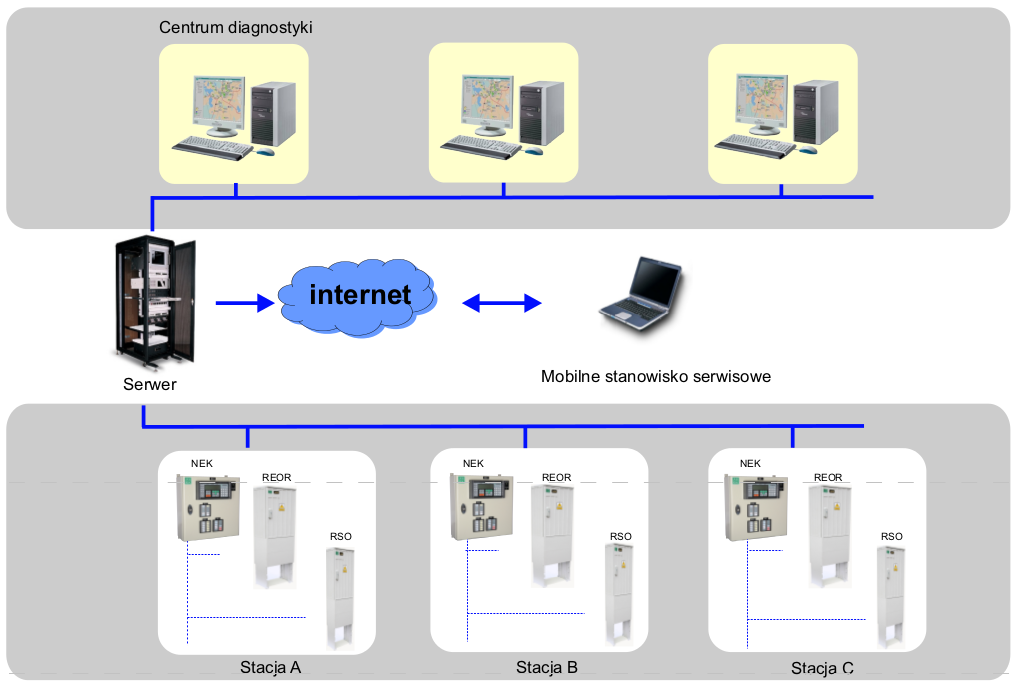
\includegraphics[height=85mm]{./img/dimacek_struktura.png}
	\caption{Struktura systemu DIMAC-EK}
	\label{fig:dimacek-scheme}
\end{figure}

\section{Standard otwarty}
DIMAC-EK został wdrożony przez firmę Arex na zamówienie Polskich Lini Kolejowych. Najpierw na kilku stacjach, a następnie system został wdrożony w całym kraju. W związku z tym nastąpiła konieczność utworzenia otwartego standardu, który jasno określa wymogi dla dostarczanych przez firmy urządzeń grzewczych. Standard ten został nazwany Standardem KHA\cite{dimacek-wytyczne}. Każda firma produkująca sprzęt zgodny z KHA może być dostawcą urządzeń dla Polskich Kolei. Na kupno urządzeń oraz administrację systemu ogłaszane są okresowo przetargi.

\section{Struktura systemu}
System DIMAC-EK składa się z następujących warstw\cite{dimacek-wytyczne}:
\begin{itemize}
\item warstwa urządzeń pomiarowych - przetworniki pogodowe,
\item warstwa urządzeń wykonawczych - grzałki elektryczne,
\item warstwa autotnomicznych rozdzielnic energetycznych - rozdzielnice oraz sterowniki EOR,
\item warstwa archiwizacji i obróbki danych - sterowniki nadrzędne NEK,
\item warstwa komunikacji systemu - sieć GSM lub LAN,
\item warstwa nadzoru i zarządzania - stanowiska diagnostyczne + serwer.
\end{itemize}


\subsection{Warstwa urządzeń pomiarowych}
Przetworniki zaopatrują sterowniki w dane pogodowe \cite{dimacek-wytyczne}. Jeden sterownik może odbierać dane z wielu przetworników. Dostępne są następujące typy przetworników pogodowych:
\begin{itemize}
\item temperatury powietrza,
\item prędkości wiatru,
\item detekcji deszczu (czujnik wilgoci),
\item detekcji śniegu,
\item temperatury szyny odniesienia (tzw. ,,zimnej''),
\item temperatury szyny ogrzewanej (tzw. ,,ciepłej''),
\item detekcji śniegu nawiewanego na rozjazd.
\end{itemize}

\subsection{Warstwa urządzeń wykonawczych}
Grzejniki można podzielić ze względu na sposób i miejsce ich montażu na torach oraz na moc. Wszystkie parametry grzejników dopuszczonych do użycia na torach znaleźć można w dokumentacji systemu dostarczanej przez PKP.


\subsection{Warstwa autonomicznych rozdzielnic energetycznych}
Rozdzielnice RESO przeznaczone są do sterowania obwodami elektrycznego ogrzewania rozjazdów oraz obwodami oświetleniowymi \cite{dimacek-wytyczne}. Poza funkcją sterującą dokonują diagnostyki obwodów oraz przetworników pomiarowych. Można o nich myśleć jako o zbiorze współpracujących ze sobą urządzeń zamontowanych w jednym miejscu. Rozdzielnice zawierają sterowniki EOR oraz moduły sterująco-diagnostyczne, które sterują pracą grzałek. Sterowniki współpracują z urządzeniami nadrzędnymi NEK, dzięki czemu pracę rozdzielnicy RESO można kontrolować z poziomu zdalnych stanowisk dyspozytorskich.

\begin{figure}[t]
	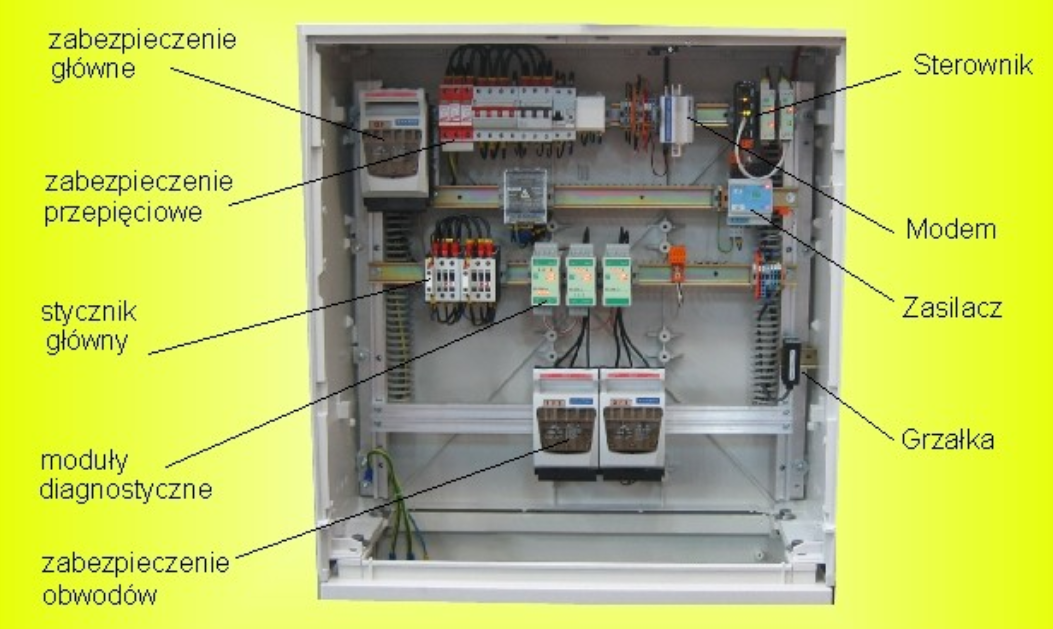
\includegraphics[height=95mm]{./img/dimacek_rozdzielnica.png}
	\caption{Budowa rozdzielnicy RESO}
	\label{fig:dimacek-reso}
\end{figure}

Rozdzielnice mogą pełnić różne funkcje w zależności od umieszczonych w nich urządzeń. Urządzenia firmy Arex są elastyczne w swej konfiguracji i działają współpracując ze sobą lub nie. Na przykład, możliwe jest poprawne działanie sterowników grzałek bez integracji z modułami diagnostycznymi, służącymi do gromadzenia oraz przesyłu danych. Dzięki standardowi KHA, w rozdzielnicy można łączyć ze sobą różne rodzaje urządzeń wyprodukowanych przez różne firmy. Wygląd oraz zawartość rozdzielnicy można zobaczyć na zdjęciu \ref{fig:dimacek-reso}.

\subsection{Warstwa archiwizacji i obróbki danych}
Sterownik nadrzędny NEK służy do zdalnego monitorowania urządzeń systemu DIMAC-EK \cite{dimacek-wytyczne}. Umożliwia on również zdalne sterowanie wszystkimi podłączonymi do niego sterownikami z poziomu jednej stacji kolejowej. Dane gromadzone przez sterownik zapisywane są w jego wewnętrznej bazie danych, którą można zarządzać z jego poziomu. Możliwy jest również przesył danych w czasie rzeczywistym do serwera przez sieć Internet. Aby zapewnić elastyczność w dostępie do danych, urządzenie NEK posiada popularne interfejsy transmisyjne:
\begin{itemize}
\item konwerter RS232-TCP/IP,
\item modem GRPS,
\item modem telefoniczny.
\end{itemize}

\subsection{Warstwa komunikacji systemu}
W granicach stacji kolejowej urządzenia komunikują się z nadrzędnym sterownikiem w standardzie CAN/DIMNET-P4\cite{dimacek-wytyczne}.
Komunikacja pomiędzy sterownikami nadrzędnymi (NEK), a serwerami realizowana jest w oparciu o sieć intranet poprzez protokół DIMNET-P5. DIMNET-P5 jest autorskim rozwiązaniem firmy Arex, który został ustanowiony otwartym standardem komunikacji pomiędzy urządzeniami energetyki kolejowej przez Polskie Linie Kolejowe. Protokół ten można stosować przy użyciu dowolnego medium danych, lecz w praktyce stosuje się sieć Internet. Schemat struktury urządzeń systemu DIMAC-EK w sieci IP znajduje się na schemacie \ref{fig:dimacek_ip}.
\begin{figure}[t]
	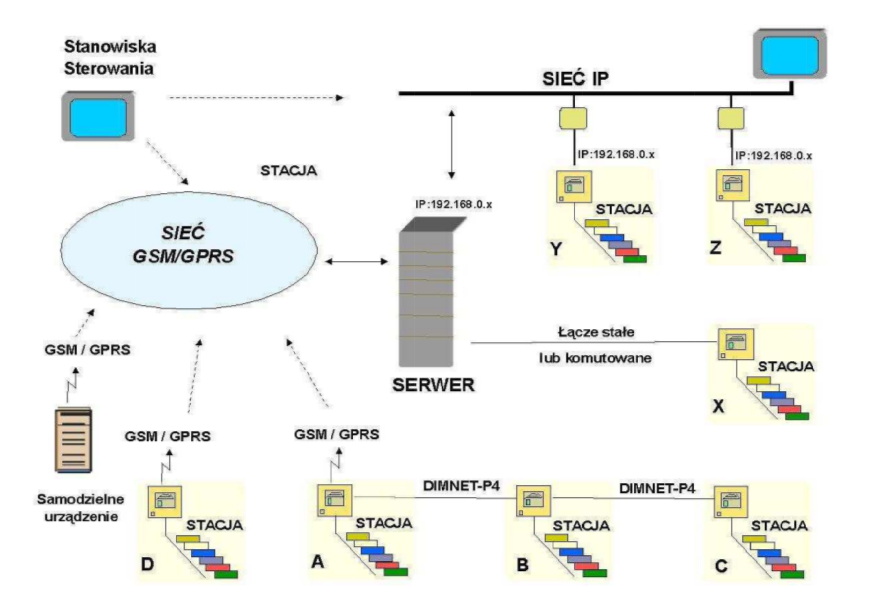
\includegraphics[height=155mm]{./img/dimacek_ip.png}
	\caption{DIMAC-EK w sieci IP}
	\label{fig:dimacek_ip}
\end{figure}


\subsection{Warstwa nadzoru i zarządzania}

Dane przesłane przez wszystkie sterowniki nadrzędne NEK gromadzone są przez serwer danych w celu archiwizacji. Ostatnim elementem systemu jest aplikacja DIVIS. Służy ona do prezentacji zgromadzonych danych w sposób zrozumiały dla osób niemających wiedzy o budowie oraz działaniu urządzeń. Aplikacja dostarcza następujące informacje:


\begin{itemize}
\item dane pogodowe w przestrzeni czasu,
\item czas grzania grzałek,
\item energia zużyta podczas pracy grzałek oraz jej koszt,
\item dane dotyczące alarmów przeciwwłamaniowych oraz przeciwpożarowych,
\item statystyka oraz analiza powyższych danych.
\end{itemize}

Należy zwrócić uwagę, iż nie ma obecnie możliwości odbioru danych z urządzeń w czasie rzeczywistym.

Rozmieszczenie elementów wszystkich warstw na stacji kolejowej zobrazowane jest na schemacie \ref{fig:dimacek-scheme}.

\begin{figure}[t]
	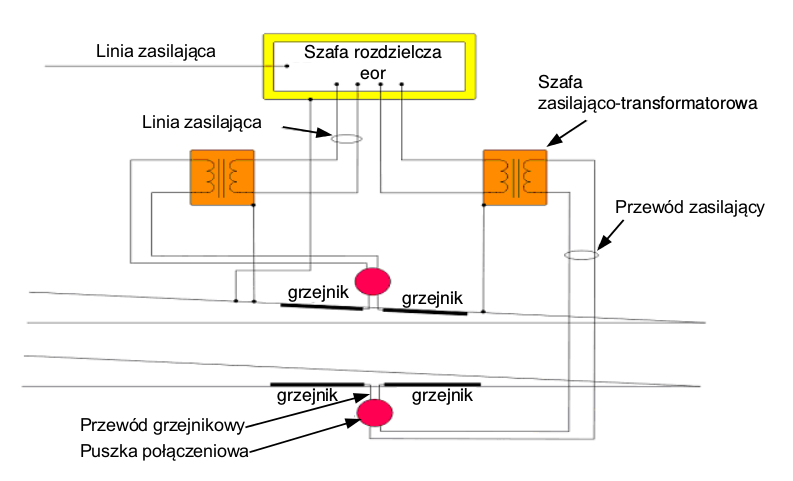
\includegraphics[height=85mm]{./img/dimacek_tory.png}
	\caption{Elementy systemu DIMAC-EK na stacji kolejowej}
	\label{fig:dimacek_tory}
\end{figure}

\section{DIMNET-P5 - protokół komunikacji}
Jednym z większych problemów w budowie systemu monitorowania ogrzewania szyn kolejowych, są duże odległości między obiektami oraz całkowity brak towarzyszącej im infrastruktury komunikacyjnej \cite{dimnetp5-spec}. Do czasu udostępnienia telefonicznych sieci komórkowych, techniczne możliwości monitorowania instalacji ogrzewania rozjazdów kolejowych stacji były znacznie ograniczone. W związku z tym, firma Arex zapoczątkowała eksperymenty nad przesyłem danych między urządzeniami za pomocą sieci GSM w 2002 roku. Jako że w tym okresie przesyłanie pakietów danych przez sieć GSM nie było tanie, należało skupić się na tym, aby metoda przesyłu była jak najbardziej oszczędna. Rozwiązaniem tego problemu jest protokół komunikacji o nazwie DIMNET-P5.

\subsection{Warstwy protokołu}
DIMNET-P5 oparty jest na wzorcu podziału usług protokołu na warstwy zgodnie z zaleceniami 7-warstwowego modelu referencyjnego ISO-OSI IEC7498 \cite{dimnetp5-spec}. W ramach protokołu zdefiniowane są jedynie warstwy powyżej transportowej (4 wg. ISO/OSI), gdyż DIMNET-P5 bazuje na powszechnie stosowanym w sieciach stosie protokołów TCP/IP i korzysta z usług protokołu TCP. Powyższymi warstwami są:
\begin{itemize}
\item warstwa kodowania - służy do wydzielania datagramów z niezawodnych strumieni bajtów w połączeniach TCP. Może również realizować opcjonalne formy kodowania lub zabezpieczania integralności danych (obsługa sum kontrolnych CRC),
\item warstwa sesji - odpowiedzialna za nawiązywanie połączenia i utrzymywanie nad nim kontroli oraz realizację wirtualnych kanałów transmisji do urządzeń w ramach jednego połączenia,
\item warstwa aplikacji - realizuje usługi komunikacyjne dostępne dla programów aplikacyjnych w stacjach końcowych.
\end{itemize}

\subsection{Jednostki i typy danych}
Urządzenia w standardzie DIMNET-P5 prezentowane są jako uporządkowany zbiór jednostek danych. Każda jednostka posiada przypisany jednoznaczny indeks, za pomocą którego identyfikowana jest zmienna \cite{dimnetp5-spec}. Każda jednostka ma również przyporządkowany typ danych. Dopuszczalne typy danych są następujące:
\begin{itemize}
\item liczba całkowita ze znakiem lub bez (8, 16, 32, 64 bity),
\item liczba zmiennoprzecinkowa (8, 16, 32, 64 bity),
\item ciąg znaków kodowanych za pomocą ASCII o określonej długości.
\end{itemize}

\subsection{Model komunikacji}
Komunikacja w DIMNET-P5 odbywa się najczęściej pomiędzy urządzeniami zdalnymi (sterownikami kontrolującymi grzałki) oraz sterownikami nadrzędnymi (NEK, serwery danych) \cite{dimnetp5-spec}. Aby zrozumieć sposób komunikacji między stacjami końcowymi należy poznać prymitywy komunikacyjne w DIMNET-P5. Określają one podstawowe interakcje występujące pomiędzy programem aplikacyjnym, a warstwą aplikacji. Są to:
\begin{itemize}
\item request - wysłanie inicjujące, wysłanie danych lub żądania obsługi,
\item indication - odbiór danych lub żądania obsługi,
\item response - wysłanie odpowiedzi na wcześniejsze żądanie obsługi,
\item confirmation - odbiór odpowiedzi potwierdzający realizację żądania.
\end{itemize}


W standardzie DIMNET-P5 możliwe są trzy sposoby komunikacji opisane poniżej.
\begin{itemize}
\item Relacja klient serwer - relacja pomiędzy pojedynczym klientem i pojedynczym serwerem. Standardowa relacja typu żądanie - odpowiedź.
\item Relacja producent-konsument - relacja między pojedynczym producentem i pojedynczym konsumentem. Producent generuje w asynchroniczny sposób komunikaty z danymi, które nie wymagają potwierdzenia. Relacja nie określa jak często lub w jakich przypadkach następuje wysłanie komunikatu.
\item Super-relacja klient-serwer - rozpoczynana przez polecenie uruchomienia procesu. Stacja, która jest serwerem potwierdza odpowiednim sygnałem sukcesu lub porażki uruchomienie procesu. W przypadku gdy odpowiedź jest pozytywna, relacja przechodzi do typu producent-konsument. Konsumentem staje się stacja typu serwer. Odstęp czasowy pomiędzy komunikatami są regulowane w całości przez proces. Polecenie zakończenia procesu powinna wysłać stacja klienta. Stacja serwer w tej sytuacji odsyła potwierdzenie otrzymania komunikatu i zatrzymuje proces. Relacja ta jest zobrazowana na schemacie \ref{fig:dimnetp5}.

	\begin{figure}[t]
		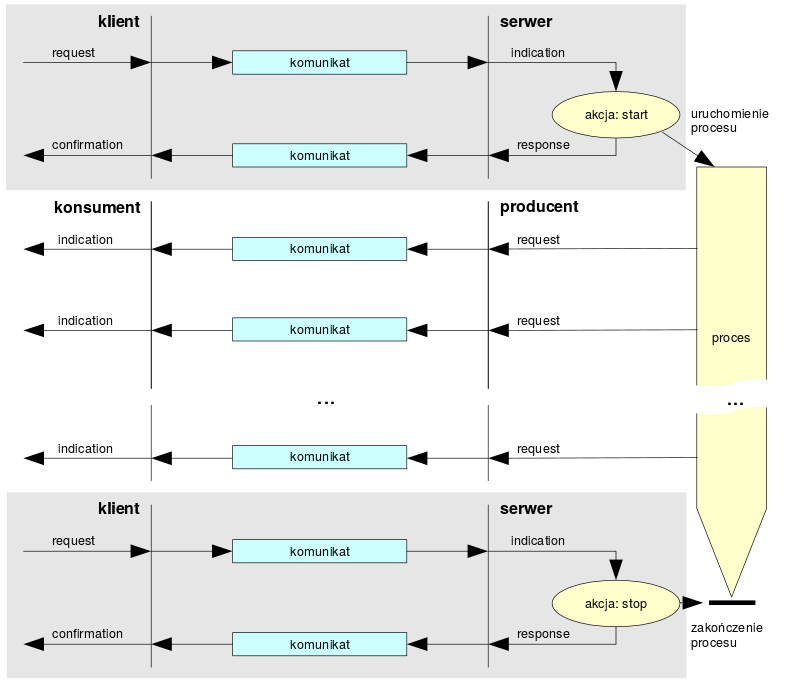
\includegraphics[height=125mm]{./img/dimnet-p5.png}
		\caption{Super-relacja serwer-klient}
		\label{fig:dimnetp5}
	\end{figure}
\end{itemize}

\subsection{Przykład zastosowania w systemie DIMAC-EK}
W systemie DIMAC-EK super-relację klient-serwer implementują na przykład\cite{dimacek-wytyczne}:
\begin{itemize}
\item serwer gromadzący dane, który jest klientem połączenia,
\item sterownik nadrzędny NEK, który pełni funkcję serwera.
\end{itemize} 
Serwer danych inicjuje połączenie, a następnie odbiera paczki z danymi od urządzenia. NEK wysyła pakiety z danymi nieustannie, do momentu sygnału zakończenia połączenia wysłanego przez serwer. Taka organizacja ma dwie podstawowe zalety: brak konieczności ciągłego odpytywania danych przez klienta oraz wysyłanie paczki danych jedynie wtedy, gdy nowe wartości różnią się od poprzednich.

\subsection{Sterowanie połączeniem}
Standard DIMNET-P5 umożliwia dodatkowe czynności sterujące połączeniem, przydatne w wielu sytuacjach. Poniżej znajduje się ich opis.
\begin{itemize}
\item Logowanie - Proces logowania jest pierwszą czynnością, która powinna zostać zapoczątkowana przez klienta nawiązującego połączenie z serwerem. Bez zakończenia tej czynności powodzeniem, stacja klienta ani serwera nie mogą wymieniać się żadnymi danymi. Podczas logowania następuje wymiana zakodowanego klucza dostępu.
\item Wylogowanie - czynność kończąca połączenie na podstawie żądania którejś ze stron połączenia. Wylogowanie może nastąpić w skutek zbyt długiego oczekiwania na pakiet utrzymujący połączenie. W takim wypadku łączność uznaje się za przerwaną.
\item Kontrola połączenia - polega na okresowej wymianie między stacjami datagramu utrzymującego połączenie, tzw. heartbeatu.
\item Synchronizacja czasu - dokonuje się jej przez datagram heartbeat. Polega na dołączeniu przez klienta do heartbeatu żądania synchronizacji. Serwer po odebraniu żądania, dołączy swój czas do kolejnego datagramu heartbeatu wysyłanego przez siebie.
\end{itemize}


\section{System Monitorowanie Urządzeń Energetycznych}
Ostatnim elementem systemu DIMAC-EK jest platforma SMUE - System Monitoringu Urządzeń Energetycznych stworzona przez firmę Arex. Jest to rozwiązanie, które współpracuje z serwerem danych archiwalnych urządzeń\cite{dimacek-wytyczne}. 

\subsection{Przyczyny powstania systemu}
W wielu przypadkach, po wdrożeniu systemu zdalnego monitoringu urządzeń na stacji, błędy w działaniu systemu uwidaczniały się dopiero po sezonie grzewczym \cite{dimacek-wytyczne}. Przyczyny problemów były następujące:
\begin{itemize}
\item nieumiejętna obsługa urządzeń,
\item awarie mechaniczne urządzeń,
\item kradzieże i zniszczenia,
\item problemy na drodze komunikacji.
\end{itemize}

Aby szybko reagować na powyższe sytuacje, stworzony została aplikacja SMUE.

\subsection{Opis aplikacji}
SMUE jest aplikacją internetową przeznaczoną dla osób, które nie muszą posiadać zaawansowanej wiedzy technicznej dotyczącej urządzeń oraz branży kolejowej\cite{dimacek-wytyczne}. Służy ona do prezentacji danych pomiarowych oraz dotyczących różnych zdarzeń przesyłanych z urządzeń zainstalowanych w terenie. SMUE analizuje je, dokonuje statystyki oraz analizy i prezentuje użytkownikowi w przejrzysty sposób. Dane gromadzone są  przez serwer Sezam i archiwizowane w bazie danych. Przykładowa strona z raportem znajduje się na obrazie \ref{fig:smue}.\\

\begin{figure}[h]
		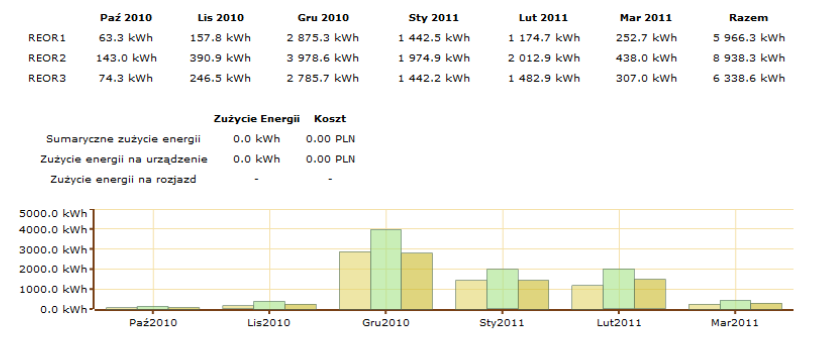
\includegraphics[height=60mm]{./img/smue.png}
		\caption{Super-relacja serwer-klient}
		\label{fig:smue}
\end{figure}

SMUE dostarcza następujące informacje:
\begin{itemize}
\item archiwalne pomiary pogodowe (temp. powietrza, wilgotność, opady atmosferyczne),
\item raporty dotyczące zużycia energii elektrycznej w różnych okresach czasu,
\item porównania dotyczące różnych stacji kolejowych na podstawie wybranych danych,
\item tabela zdarzeń urządzeń (rozpoczęcie, zakończenie grzania, włamania, utrata połączenia, usterki).
\end{itemize}

\section{Podsumowanie}
System DIVIS-EK jest kompletnym systemem służącym do monitorowania urządzeń energetyki kolejowej. Posiada wszelkie możliwe komponenty do komunikowania, kontrolowania oraz diagnozowania urządzeń. Rozwiązanie zawiera również narzędzie do analizowania danych zbieranych przez system. Warto jednak zauważyć, iż nie istnieje rozwiązanie, które byłoby w stanie zaprezentować w przejrzysty sposób dane z urządzeń w czasie rzeczywistym. Praktyczna część niniejszej pracy została poświęcona temu problemowi.